\documentclass[aspectratio=169, 11pt]{beamer}

% ====== Theme ======
\usetheme{Madrid}
\definecolor{CityUBlue}{RGB}{0, 51, 102}
\definecolor{CityULightBlue}{RGB}{0, 102, 179}
\definecolor{CityUGold}{RGB}{198, 163, 0}
\definecolor{CityUGray}{RGB}{90, 90, 90}
\usecolortheme[named=CityUBlue]{structure}
\setbeamercolor{title}{fg=white, bg=CityUBlue}
\setbeamercolor{frametitle}{fg=white, bg=CityUBlue}
\setbeamercolor{block title}{bg=CityUBlue, fg=white}
\setbeamercolor{block body}{bg=CityUBlue!10, fg=black}
\setbeamercolor{block title alerted}{bg=CityUGold, fg=white}
\setbeamercolor{block body alerted}{bg=CityUGold!15, fg=black}
\setbeamercolor{item}{fg=CityUBlue}
\setbeamercolor{subitem}{fg=CityULightBlue}
\setbeamercolor{alerted text}{fg=CityUGold!90!black}

% ====== Packages ======
\usepackage[T1]{fontenc}
\usepackage{lmodern}
\usepackage{booktabs}
\usepackage{graphicx}
\usepackage{hyperref}
\usepackage{amsmath, amssymb}
\usepackage{tikz}
\usetikzlibrary{positioning, arrows.meta, calc, shapes.geometric, fit}
\usepackage{appendixnumberbeamer}

% ====== Settings ======
\setbeamertemplate{navigation symbols}{}
\setbeamertemplate{itemize item}{\color{CityUBlue}$\blacktriangleright$}
\setbeamertemplate{itemize subitem}{\color{CityULightBlue}$\bullet$}
\graphicspath{{figures/}{../../Figures used in slides/}}

% ====== Metadata ======
\title[EF8083 Lecture 6]{PhD Lecture in Behavioral Asset Pricing:\\ Memory and Markets}
\subtitle{A New Psychological Primitive for Beliefs and Prices}
\author[F.\ W.\ Li]{Frank Weikai Li}
\institute[CityU]{Associate Professor of Finance\\City University of Hong Kong}
\date{}

% ==============================================================================
\begin{document}
% ==============================================================================

% --- Slide 1: Title ---
\begin{frame}[plain]
\titlepage
\end{frame}

% --- Slide 2: Motivation ---
\begin{frame}{Why Memory?}
\begin{itemize}
\item \textbf{Beliefs are the central object of asset pricing.}
  \begin{itemize}
  \item What investors expect about future returns drives prices, volume, and bubbles
  \item Standard models assume investors \emph{use} the full history of information efficiently
  \end{itemize}
\item \textbf{But human memory is not a faithful archive.}
  \begin{itemize}
  \item Recall is \emph{reconstructive} and \emph{cue-dependent}: what comes to mind depends on the current context
  \item Psychologists have known this for 50 years (Tulving \& Thomson, 1973; Kahana, 2012)
  \end{itemize}
\item \textbf{A new literature asks: does this matter for markets?}
  \begin{itemize}
  \item If beliefs are formed from \emph{recalled} (not actual) experiences, mispricing follows
  \item Memory is distinct from --- and upstream of --- sentiment, attention, and extrapolation
  \end{itemize}
\end{itemize}
\vfill
\begin{block}{This lecture}
Four recent papers make memory a first-class primitive in behavioral finance: from the lab, to individual investors, to the cross-section of stocks, to market prices.
\end{block}
\end{frame}

% --- Slide 3: Roadmap ---
\begin{frame}{Roadmap}
\begin{enumerate}
\item \textbf{Psychology foundation} --- associative memory and cue-dependent retrieval
\item \textbf{Theory} --- from recalled experiences to biased beliefs
\item \textbf{Causal lab evidence} --- Enke, Schwerter \& Zimmermann (2024, \textit{JFE})
\item \textbf{Field evidence: individual investors} --- Jiang, Liu, Peng \& Yan (2025, \textit{QJE})
\item \textbf{Marketwide evidence} --- Charles \& Sui (2024, working paper)
\item \textbf{Memory moves prices} --- Charles (2024, \textit{RFS})
\item \textbf{Synthesis, open questions, and a research agenda}
\end{enumerate}
\vfill
\begin{alertblock}{Guiding question}
Does memory provide a \emph{microfoundation} for the beliefs and prices we see --- overreaction, extrapolation, comovement, crisis echoes?
\end{alertblock}
\end{frame}

% ==============================================================================
\section{Psychology Foundation}
% ==============================================================================

\begin{frame}{Associative Memory: The Psychology}
\begin{itemize}
\item \textbf{Memory is not a tape recorder.} Recall is \emph{cue-dependent}: a present stimulus (the \emph{cue}) retrieves past episodes that resemble it (Tulving \& Thomson, 1973; Kahana, 2012)
\item \textbf{Four robust laws of cued recall} (Kahana, 2012):
  \begin{itemize}
  \item \emph{Similarity} --- episodes similar to the cue are retrieved more easily
  \item \emph{Interference} --- a focal episode is harder to retrieve when many similar episodes compete
  \item \emph{Contiguity} --- episodes experienced close in time tend to be co-retrieved
  \item \emph{Recency} --- recent episodes are more available
  \end{itemize}
\item \textbf{Key implication for finance:}
  \begin{itemize}
  \item Today's market return / news / context acts as a \emph{cue}
  \item It asymmetrically retrieves \emph{congruent} past experiences
  \item Beliefs are built from this \emph{biased sample} of memory, not from the full history
  \end{itemize}
\end{itemize}
\end{frame}

\begin{frame}{From Memory to Beliefs: A Two-Step Mechanism}
\begin{columns}[T]
\begin{column}{0.52\textwidth}
\textbf{Step 1 --- Cued recall.}\\[0.3em]
Today's context $\kappa_t$ retrieves past experiences $\{e\}$ with probability
\[
r(e,\kappa_t) \;=\; \frac{S(e,\kappa_t)}{\sum_{e'} S(e',\kappa_t)}, \qquad S(e,\kappa_t)\in[0,1]
\]
where $S$ is a similarity kernel (e.g.\ cosine).
\\[0.6em]
\textbf{Step 2 --- Simulation.}\\[0.3em]
The investor averages retrieved experiences to \emph{simulate} a future return distribution, then forecasts from it.
\end{column}
\begin{column}{0.46\textwidth}
\begin{block}{Memory-based expectation}
\[
\mathbb{E}^{\text{mem}}[r_{t+1}] \;=\; \sum_{e} r(e,\kappa_t)\, r(e)
\]
Beliefs are a \emph{recall-weighted} average of past returns --- not a time-weighted one.
\end{block}
\vspace{0.4em}
\footnotesize
\textbf{Foundations:} Bordalo, Burro, Coffman, Gennaioli \& Shleifer (2025, \textit{RES}); Wachter \& Kahana (2024); Gennaioli \& Shleifer (2018).
\\[0.3em]
\textbf{Punchline:} \emph{extrapolation} and \emph{recency} \emph{emerge} from this mechanism --- they are not assumed as primitives.
\end{column}
\end{columns}
\end{frame}

\begin{frame}{How Memory Differs from Neighbouring Concepts}
\begin{itemize}
\item \textbf{vs.\ Extrapolation} (Greenwood \& Shleifer, 2014; Barberis et al., 2018):\\
  extrapolation is a \emph{reduced-form} fact; memory is its \emph{mechanism}
\item \textbf{vs.\ Experience effects} (Malmendier \& Nagel, 2011, 2016):\\
  experience weights past returns by \emph{fixed} exponential decay; memory weights them by \emph{context-dependent} similarity --- so recall \emph{spikes} during crises
\item \textbf{vs.\ Sentiment} (Baker \& Wurgler, 2006):\\
  sentiment is a market-wide mood; memory is a within-inferior cognitive process that \emph{produces} the belief input
\item \textbf{vs.\ Attention} (Barber \& Odean, 2008; Hirshleifer, Lim \& Teoh, 2009):\\
  attention selects \emph{which external} stimuli to process; memory generates \emph{internal} cues from the past
\end{itemize}
\vfill
\begin{block}{Position in the literature}
Memory sits \emph{upstream} --- it shapes the beliefs that extrapolation, sentiment, and attention then act on.
\end{block}
\end{frame}

% ==============================================================================
\section{Causal Lab Evidence}
% ==============================================================================

\begin{frame}{Enke, Schwerter \& Zimmermann (2024, JFE): Design}
\begin{itemize}
\item \textbf{Question:} does associative recall \emph{cause} overreaction in expectations and prices?
\item \textbf{Setup:} three pre-registered lab experiments
  \begin{itemize}
  \item Subjects observe signals about a binary state $\theta\in\{G,B\}$ over two periods
  \item First period: $k\in\{0,\ldots,4\}$ signals. Second period: one signal $s_{k+1}$
  \item Each signal is embedded in a \emph{context} (a background image / narrative)
  \end{itemize}
\item \textbf{Manipulation (within-subject):}
  \begin{itemize}
  \item \textbf{Cue:} signals congruent in sign share the same context $\Rightarrow$ cue facilitates recall
  \item \textbf{NoCue:} contexts never repeat $\Rightarrow$ no associative retrieval
  \end{itemize}
\item \textbf{Identification:} $z$ = number of first-period signals \emph{congruent} with $s_{k+1}$ is random; the Bayesian benchmark is a coefficient of \emph{exactly 1} on $s_{k+1}$
\item \textbf{Three experiments:} Beliefs (incentivized), Recall (surprise elicitation), Betting Market (parimutuel, groups of 3)
\end{itemize}
\end{frame}

\begin{frame}[shrink=5]{Enke et al.\ (2024): Results}
\begin{columns}[T]
\begin{column}{0.50\textwidth}
\textbf{Beliefs overreact only when memory is cued.}
\begin{itemize}
\item Coefficient on $s_{k+1}$: \textbf{1.20} in Cue vs.\ $\approx$\textbf{1.0} in NoCue
\item Treatment $\times$ signal interaction: \textbf{0.61}*** (s.e.\ 0.15) --- $>$80\% larger response
\item Rises monotonically in $z$ (\# congruent signals)
\item Null when $z=0$ --- rules out ``better recall in general''
\end{itemize}
\textbf{Mechanism confirmed.}\\
Subjects retrieve \emph{congruent} first-period signals in Cue, not incongruent ones.
\end{column}
\begin{column}{0.48\textwidth}
\begin{alertblock}{Markets do not attenuate}
Market-price overreaction (\textbf{0.65}***) $\approx$ individual-belief overreaction (\textbf{0.61}***).

Self-selection fails to dampen prices: the lab market \emph{aggregates} the bias rather than correcting it.
\end{alertblock}
\vspace{0.3em}
\footnotesize
\textbf{Takeaway:} a clean causal link from associative recall $\to$ belief overreaction $\to$ price overreaction. Narratives move prices through \emph{retrieval}, not through information.
\end{column}
\end{columns}
\end{frame}

% ==============================================================================
\section{Field Evidence: Individual Investors}
% ==============================================================================

\begin{frame}{Jiang, Liu, Peng \& Yan (2025, QJE): Design}
\begin{itemize}
\item \textbf{Question:} do investors form return expectations by selectively \emph{recalling} past experiences --- and do recalled (not actual) experiences drive beliefs and trading?
\item \textbf{Data:}
  \begin{itemize}
  \item Nationally representative survey of $\sim$\textbf{17,000 Chinese retail investors}, late 2021
  \item Survey rolled out in three waves over six weeks $\Rightarrow$ plausibly exogenous variation in daily market returns (the \emph{cue})
  \item Merged subsample ($\sim$\textbf{5,154}) with administrative brokerage records
  \end{itemize}
\item \textbf{Two recall elicitations:}
  \begin{itemize}
  \item \textbf{FreeRecall:} ``recall a market episode that first comes to mind'' (Neutral / Happy / Painful)
  \item \textbf{ProbedRecall:} recall own return over horizons from yesterday to 5 years
  \end{itemize}
\item \textbf{Identification:} survey-day market return as the cue; respondents instructed not to consult external sources
\item \textbf{Validity:} recalled vs.\ actual market-return correlation $= 0.57$
\end{itemize}
\end{frame}

\begin{frame}[shrink=5]{Jiang et al.\ (2025): Results}
\begin{itemize}
\item \textbf{Cued recall.} +1pp survey-day market return $\Rightarrow$ +\textbf{2.5--4.1pp} recalled episode return; +\textbf{52bps} recalled own return (yesterday), +\textbf{113bps} (past month) --- \emph{after controlling for actual own return}
\item \textbf{Recall $\to$ beliefs.} Moving recalled past-month own return from 25th to 75th percentile raises 1-month expectation by \textbf{0.7pp} and 1-year expectation by \textbf{1.8pp}
\item \textbf{Recalled dominates actual.} In horse races, recalled experiences \emph{out-explain} actual experiences; controlling for recalls \emph{weakens} the actual-experience--expectations link
\item \textbf{Horizon dependence.} 1-year forecasts weight recalled 1-year returns; 1-month forecasts weight recalled 1-month returns
\item \textbf{Memory $\to$ trading.} +1pp memory-induced own-return expectation raises net buying by \textbf{71 RMB} (survey day) and \textbf{1,141 RMB} (next month) --- far larger than raw expectations
\end{itemize}
\vfill
\begin{block}{Punchline}
``A rising market prompts investors to recall their past experiences more positively, leading to more optimistic forecasts'' --- \emph{extrapolation as a memory artifact}.
\end{block}
\end{frame}

% ==============================================================================
\section{Marketwide Evidence}
% ==============================================================================

\begin{frame}{Charles \& Sui (2024): Marketwide Memory}
\begin{itemize}
\item \textbf{Question:} can the laws of associative memory, applied at scale to the cross-section of stocks over decades, explain investor beliefs and trading?
\item \textbf{The measure:} for each stock-month, reconstruct a \emph{recall probability} over the past 180 months using
\[
r(e,\kappa_t) \;=\; \frac{S(e,\kappa_t)}{\sum_{e'} S(e',\kappa_t)}, \qquad S(e,\kappa_t) = \tfrac{1}{2}\bigl[\cos(e,\kappa_t) + 1\bigr]
\]
where $e$ is a past month encoded by stock-level, firm-level, and macro features
\item \textbf{Key features of the measure:}
  \begin{itemize}
  \item \emph{Similarity} and \emph{interference} both operate --- interference makes recall \emph{context-dependent}
  \item \emph{Recency emerges endogenously} --- no exponential decay assumed
  \item \emph{Crisis echoes}: COVID-2020 cues 2008; 2008 cues 2001; 1979 cues 1973 --- patterns pure extrapolation \emph{cannot} produce
  \end{itemize}
\item \textbf{Scope:} CRSP stocks listed $\geq$15 years, 1966--2021
\end{itemize}
\end{frame}

\begin{frame}[shrink=10]{Charles \& Sui (2024): Validation and Findings}
\begin{columns}[T]
\begin{column}{0.50\textwidth}
\textbf{Validates against real recall.}
\begin{itemize}
\item Correlation \textbf{0.88} (rank 0.79) with mentions in earnings-call transcripts (Refinitiv, 2001--2021)
\item 1pp higher recall prob $\Rightarrow$ \textbf{67pp} higher mention probability; exponential-decay weight becomes insignificant
\end{itemize}
\textbf{Explains beliefs.}
\begin{itemize}
\item Corr \textbf{0.67} with Gallup bullish-minus-bearish; 1 SD $\Rightarrow$ \textbf{14.5pp} more bullish investors
\item Survives controls for past-12m and 5-year exp-weighted return
\end{itemize}
\end{column}
\begin{column}{0.48\textwidth}
\textbf{Explains higher moments.}
\begin{itemize}
\item Memory-based volatility tracks option-implied vol (1 SD $\Rightarrow$ 59\% of SD); time-series version explains VIX
\end{itemize}
\textbf{Explains trading.}
\begin{itemize}
\item For the same realized gain, raising recall prob 0$\to$10\% raises repurchase likelihood by \textbf{0.11pp} ($\sim$22\% of unconditional rate)
\end{itemize}
\end{column}
\end{columns}
\vfill
\begin{block}{Distinction}
Recency is not assumed --- it \emph{emerges} from similarity and interference. Crisis-echo spikes are the signature of memory, not extrapolation.
\end{block}
\end{frame}

% ==============================================================================
\section{Memory Moves Prices}
% ==============================================================================

\begin{frame}{Charles (2024, RFS): Memory Moves Markets}
\begin{itemize}
\item \textbf{Question:} can \emph{internally generated} attention --- driven by associative memory links between firms --- distort stock prices, separately from any external attention stimulus?
\item \textbf{The association:} two firms that announced earnings on the \emph{same day} last quarter become \emph{associated in memory} (shared encoding context)
\item \textbf{The cue:} this quarter, when only firm A announces, the event cues recall of firm B $\Rightarrow$ internally generated attention to B $\Rightarrow$ retail net buying (Barber \& Odean, 2008) $\Rightarrow$ price pressure
\item \textbf{Identification:} Noh, So \& Verdi (2021) ``pattern firms'' --- firms following rigid announcement-timing rules (e.g.\ first Thursday of month) for $\geq$3 years. Calendar rotations exogenously shift announcement dates, creating plausibly random overlaps
\item \textbf{Sample:} 2005--2019, $\sim$16.5M firm-days; CRSP/Compustat/I/B/E/S; retail order imbalance from TAQ
\item \textbf{Controls:} own-EA dummies, 8-K filings, RavenPack sentiment/volume, day FE, firm-year-quarter FE; cueing firms in \emph{different} TNIC industry, not vertically related, no shared analysts
\end{itemize}
\end{frame}

\begin{frame}[shrink=5]{Charles (2024): Price Dynamics}
\begin{columns}[T]
\begin{column}{0.52\textwidth}
\textbf{Cue $\to$ price.}
\begin{itemize}
\item Baseline: cue $\Rightarrow$ \textbf{+4bps} $[t,t+1]$, \textbf{+8bps} $[t,t+10]$ (full controls, 1\% sig.)
\item \textbf{Builds over $\sim$2 weeks, then fully reverses over $\sim$3 weeks} --- zero by $\sim$25 trading days
\item Inconsistent with fundamental information; signature of attention-driven mispricing
\end{itemize}
\textbf{Retail-driven.}
\begin{itemize}
\item Retail order imbalance positive and significant over $[t,t+10]$
\item Effect concentrated in \textbf{small cued firms}
\item Stronger post-2015 (Robinhood era): trading strategy alpha \textbf{+69.3bps} over $[t,t+10]$, $\sim$16\% annualized
\end{itemize}
\end{column}
\begin{column}{0.46\textwidth}
\begin{alertblock}{Internal vs external attention}
Memory associations inside an investor's mind are an \emph{internal} source of attention, distinct from all external sources previously studied (news, volume, extreme returns).
\end{alertblock}
\vspace{0.3em}
\footnotesize
\textbf{Mechanism checks:} effect stronger when encoding-day volume high; \emph{extremely negative} co-surprises yield \emph{negative} response (similarity). Interference and contiguity directionally consistent.
\\[0.3em]
\textbf{Limits to arbitrage:} small stocks, shorting costs --- exactly where mispricing survives.
\end{column}
\end{columns}
\end{frame}

% ==============================================================================
\section{Synthesis}
% ==============================================================================

\begin{frame}{A Unified Framework: From Context to Prices}
\vspace{-0.2em}
\centering
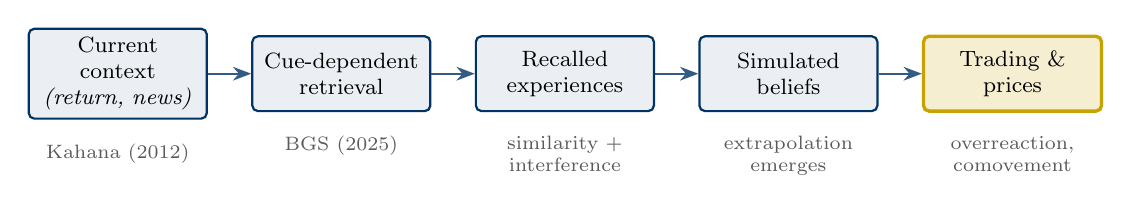
\begin{tikzpicture}[
  node distance=0.45cm and 0.55cm,
  every node/.style={font=\footnotesize},
  box/.style={rectangle, draw=CityUBlue, thick, rounded corners=2pt, fill=CityUBlue!8, text width=2.05cm, align=center, minimum height=0.95cm, inner sep=3pt},
  resultbox/.style={rectangle, draw=CityUGold, very thick, rounded corners=2pt, fill=CityUGold!18, text width=2.05cm, align=center, minimum height=0.95cm, inner sep=3pt},
  arr/.style={-Stealth, thick, CityUBlue!80}
]
\node[box] (context) {Current context\\ \textit{(return, news)}};
\node[box, right=of context] (cue) {Cue-dependent\\ retrieval};
\node[box, right=of cue] (recall) {Recalled\\ experiences};
\node[box, right=of recall] (belief) {Simulated\\ beliefs};
\node[resultbox, right=of belief] (price) {Trading \&\\ prices};
\draw[arr] (context) -- (cue);
\draw[arr] (cue) -- (recall);
\draw[arr] (recall) -- (belief);
\draw[arr] (belief) -- (price);

\node[below=0.18cm of context, text=CityUGray, font=\scriptsize, text width=2.05cm, align=center] {Kahana (2012)};
\node[below=0.18cm of cue, text=CityUGray, font=\scriptsize, text width=2.05cm, align=center] {BGS (2025)};
\node[below=0.18cm of recall, text=CityUGray, font=\scriptsize, text width=2.05cm, align=center] {similarity + interference};
\node[below=0.18cm of belief, text=CityUGray, font=\scriptsize, text width=2.05cm, align=center] {extrapolation emerges};
\node[below=0.18cm of price, text=CityUGray, font=\scriptsize, text width=2.05cm, align=center] {overreaction, comovement};
\end{tikzpicture}
\vspace{0.6em}
\begin{columns}[T]
\begin{column}{0.48\textwidth}
\textbf{Four papers as building blocks:}
\begin{itemize}
\item \textbf{ESZ (2024):} causal link, lab
\item \textbf{JLPY (2025):} recalled $>$ actual, field
\end{itemize}
\end{column}
\begin{column}{0.50\textwidth}
\begin{itemize}
\item \textbf{Charles \& Sui (2024):} scale to cross-section
\item \textbf{Charles (2024):} memory moves prices
\end{itemize}
\end{column}
\end{columns}
\vfill
\footnotesize\centering Memory is the \emph{mechanism}; extrapolation, comovement, and crisis echoes are the \emph{consequences}.
\end{frame}

\begin{frame}[shrink=5]{What Memory Explains --- and What It Doesn't (Yet)}
\begin{columns}[T]
\begin{column}{0.50\textwidth}
\textbf{Explains}
\begin{itemize}
\item Overreaction to cued signals (ESZ)
\item Return extrapolation as a recall artifact (JLPY)
\item Recency \emph{and} crisis-echo spikes (Charles \& Sui)
\item Repurchase and disposition-style trading
\item Internally-generated comovement \& price pressure (Charles)
\item Why lab designs (no memory) find \emph{under}reaction while field finds \emph{over}reaction
\end{itemize}
\end{column}
\begin{column}{0.48\textwidth}
\textbf{Doesn't (yet)}
\begin{itemize}
\item Aggregation: how individual recall becomes market price
\item Institutional / sophisticated investors
\item Long-horizon dynamics and bubbles/crashes
\item Trauma vs.\ contextual memory
\item Interaction with sentiment and limits to arbitrage
\item Welfare and structural pricing implications
\end{itemize}
\end{column}
\end{columns}
\vfill
\begin{alertblock}{Open questions for PhD research}
How does memory aggregate? Do institutions remember differently? Can memory-based measures \emph{predict} returns out of sample? These are first-order questions --- and largely open.
\end{alertblock}
\end{frame}

\begin{frame}{Takeaways}
\begin{enumerate}
\item \textbf{Memory is a new primitive.} Beliefs are built from \emph{recalled}, not actual, experiences --- and recall is cue-dependent, associative, and biased
\item \textbf{The mechanism is two-step.} Cued retrieval $+$ simulation. Extrapolation and recency \emph{emerge} rather than being assumed
\item \textbf{It scales.} From the lab (ESZ) to 17K investors (JLPY) to the cross-section over 55 years (Charles \& Sui) to prices (Charles)
\item \textbf{Markets reflect memory.} Price overreaction in the lab is as large as belief overreaction; in the field, memory cues move prices and \emph{reverse}
\item \textbf{Memory is upstream.} It shapes the belief input that extrapolation, sentiment, and attention then act on
\item \textbf{Rich research agenda.} Aggregation, institutions, long horizons, trauma, out-of-sample prediction --- all open
\end{enumerate}
\vfill
\begin{block}{Bottom line}
Memory gives behavioral finance a \emph{microfoundation} for beliefs --- and a new lever for understanding prices.
\end{block}
\end{frame}

% ==============================================================================
\section*{References}
% ==============================================================================

\begin{frame}{Core References}
\scriptsize
\begin{itemize}
\item Enke, B., Schwerter, F., \& Zimmermann, F.\ (2024). Associative memory, beliefs and market interactions. \textit{Journal of Financial Economics}, 157, 103853.
\item Jiang, Z., Liu, H., Peng, C., \& Yan, H.\ (2025). Investor memory and biased beliefs: Evidence from the field. \textit{Quarterly Journal of Economics}, qjaf035.
\item Charles, C., \& Sui, P.\ (2024). Marketwide memory. Working paper, LSE \& CUHK-Shenzhen.
\item Charles, C.\ (2024). Memory moves markets. \textit{Review of Financial Studies}, hhae086.
\end{itemize}
\vspace{0.4em}
\textbf{Foundational psychology \& theory}
\begin{itemize}
\item Kahana, M.\ (2012). \textit{Foundations of Human Memory}. Oxford University Press.
\item Tulving, E., \& Thomson, D.\ (1973). Encoding specificity and retrieval processes in episodic memory. \textit{Psychological Review}, 80(5), 352--373.
\item Bordalo, P., Burro, G., Coffman, K., Gennaioli, N., \& Shleifer, A.\ (2025). Memory and probability. \textit{Review of Economic Studies}.
\item Gennaioli, N., \& Shleifer, A.\ (2018). \textit{A Crisis of Beliefs: Investor Psychology and Financial Fragility}. Princeton University Press.
\item Wachter, J., \& Kahana, M.\ (2024). A retrieved-context model of financial decisions.
\end{itemize}
\vspace{0.3em}
\textbf{Related behavioural finance}
\begin{itemize}
\item Malmendier, U., \& Nagel, S.\ (2011, 2016). Depression babies; learning from inflation.
\item Greenwood, R., \& Shleifer, A.\ (2014). Expectations of returns and expected returns.
\item Barber, B., \& Odean, T.\ (2008). All that glitters.
\item Baker, M., \& Wurgler, J.\ (2006). Investor sentiment and the cross-section of stock returns.
\end{itemize}
\end{frame}

\end{document}
